\documentclass[11pt,letterpaper]{article}

% --- packages (Econometrica-flavored single-column article) ---
\usepackage[margin=1in]{geometry}
\usepackage{amsmath,amssymb,amsthm}
\usepackage{booktabs}
\usepackage{array}
% siunitx not installed locally — provide a lightweight \num{} fallback.
% Accepts plain numbers (passed through) and scientific notation written as
% \num{1.535e-4} -> 1.535 \times 10^{-4}. We rely on \enum below for sci
% formatting and keep \num for plain pass-through.
\providecommand{\num}[1]{\ensuremath{#1}}
\providecommand{\enum}[2]{\ensuremath{#1 \times 10^{#2}}}
\usepackage{natbib}
\usepackage{hyperref}
\usepackage{url}
\usepackage{enumitem}
\usepackage{xcolor}
\usepackage{graphicx}
\usepackage{caption}

\hypersetup{colorlinks=true,linkcolor=black,citecolor=blue,urlcolor=blue}

% Slightly looser tolerance to avoid \texttt-with-underscore overfulls.
\tolerance=2000
\emergencystretch=3em

% --- math conveniences ---
\newcommand{\Var}{\operatorname{Var}}
\newcommand{\Cov}{\operatorname{Cov}}
\newcommand{\dln}{\Delta\ln}
\newcommand{\sbe}{s_{\mathrm{be}}}
\newcommand{\sexp}{s_{\mathrm{exp}}}
\newcommand{\Cfx}{\mathrm{FX}}

% --- theorem-like environments for assumptions ---
\newtheoremstyle{assumption}{1em}{1em}{\itshape}{}{\bfseries}{.}{.5em}{}
\theoremstyle{assumption}
\newtheorem{assumption}{Assumption}

\title{Detecting Q-Dominance Ex-Ante for Streamed-Liability Convex Hedges:\\[0.3em]
  An FX-Variance-Share Sensitivity Surface Methodology\\[0.6em]
  \large Section 5 --- E10 GSPS Application}
\author{Abrigo Analytics --- Iteration \texttt{e10\_gsps\_v0.7}}
\date{2026-05-21}

\begin{document}
\maketitle

\begin{abstract}
We propose a methodology for detecting, ex-ante and from public-source data,
whether a streamed-liability convex hedge addresses the dominant variance
vector of a target cohort's cost stream. The methodology is built around an
exact three-way log-variance decomposition of the cost-stream identity
$\Cfx_t \cdot p \cdot Q_t$ into FX, Q, and covariance components on a common
daily gapped grid; an FX-variance-share sensitivity surface evaluated on a
log-spaced grid across an anchored Q-volume range; and a six-input
collectively-exhaustive descriptive verdict ladder consuming surface,
material-gap, simulator-anchored, Q-variance-dominance, interior-crossing, and
data-visibility flags. The methodology emits one of
\textsc{Surface-Produced}, \textsc{Partial}, or \textsc{Non-Retirement}.
Applied to the E10 representative Web3 data-analyst cohort over a 5-currency
panel (COP, BRL, EUR, GBP, NGN; 150 monthly cells; 2023-11 to 2026-04), the
empirical FX-variance share sits approximately 3.21 decades below the
ex-ante-pinned break-even $\sbe = 0.25$ at every grid point on the anchored
$[28, 130]$ queries/month range; all five pre-committed sensitivity arms
remain concordant; the verdict is \textsc{Non-Retirement}, subtype
\texttt{q\_dominance}. The methodology contribution survives the specific
verdict: it correctly identifies a (cohort, instrument) pair for which the
convex FX hedge addresses the wrong variance vector, and provides an
auditable Tier-2-frozen trail from raw central-bank data to the descriptive
verdict.
\end{abstract}

% =====================================================================
\section{Motivation and contribution claim}
\label{sec:e10-motivation}

A growing literature on permissionless on-chain convex hedges constructs
instruments aimed at protecting cohort cash flows from particular sources of
volatility \citep{LambertLyonsJiao2022,Maymin2026}. The construction step ---
how to size, price, and statically replicate a convex payoff
\citep{Lambert2022Panoptic} --- has matured. What has not matured is the
\emph{detection} step that must precede construction: does the cohort's
cost-stream variance actually load on the variance vector the proposed
instrument prices, or does it load on a different vector against which the
instrument provides no payoff?

This section contributes a methodology for detecting Q-dominance ex-ante from
public-source data alone. We define Q-dominance as the empirical state in
which the variance of the cohort's stochastic activity intensity ($Q$)
dominates the variance of the FX leg in the cost-stream log-variance
decomposition. Under Q-dominance, a convex FX hedge addresses the wrong
variance vector for the cohort and is descriptively unsuited to the (cohort,
instrument) pair --- regardless of how well-constructed the hedge itself is.

The methodology is delivered as a sequence of three ex-ante-pinned objects:
(i) an exact three-way log-variance decomposition operating on a common daily
gapped grid; (ii) an FX-variance-share sensitivity surface evaluated on a
log-spaced grid spanning an anchored Q-volume range; (iii) a collectively
exhaustive descriptive verdict ladder consuming six input flags. The
contribution is the detection step --- it is independent of, and survives,
any particular cohort's verdict.

\paragraph{Posture.}
Throughout this section we adopt a \emph{descriptive} posture: no inferential
$\beta$ claim is made, no $p$-value is computed, no null hypothesis is
rejected. The objects emitted are surfaces, decompositions, and verdict
classifications under a stated calibration; they are read against
ex-ante-pinned thresholds. The descriptive posture is the load-bearing
anti-fishing safeguard \citep{AbrigoSpecE10v07}.

% =====================================================================
\section{Setup and assumptions}
\label{sec:e10-setup}

The methodology is stated as five formal assumptions.

\begin{assumption}[Cohort]\label{ass:A1}
The cohort pays a continuous-stream liability of the form
\begin{equation}
  C_t \;=\; Q_t \cdot p \cdot \Cfx_t,
  \label{eq:cost-identity}
\end{equation}
where $Q_t$ is the daily query volume (an x402-priceable activity intensity
measured in queries per day), $p$ is a verified flat unit price
($p = \$0.01$ USDC per query in E10, x402-protocol-verified), and $\Cfx_t$ is
the daily local-currency-per-USD exchange rate published by a sovereign
central bank.
\end{assumption}

\begin{assumption}[Data anchors]\label{ass:A2}
The activity-intensity process $Q_t$ is empirically anchored to a NON-FANTASY
observed trace: in E10, 214 genuine Claude Code transcript tool calls
extracted from on-disk session logs (daily VMR $\approx 20$, decisively
overdispersed). The FX panels $\Cfx_t$ are sourced from public central-bank
feeds: Banrep TRM (COP), BCB Olinda OData PTAX (BRL), ECB Data Portal SDW
(EUR), BoE IADB (GBP), CBN Gateway (NGN). All five series are free,
machine-readable, daily, and re-verified per-currency at the data-visibility
gate.
\end{assumption}

\begin{assumption}[Panel construction]\label{ass:A3}
A balanced panel of $(\text{currency} \times \text{month})$ cells is
constructed on a daily gapped grid: zero-Q days are dropped from the
$\dln \Cfx$ and $\dln Q$ series on the SAME surviving index per cell
(forced by the log domain --- $\dln(0)$ is undefined). In E10 the panel
comprises 5 currencies $\times$ 30 months $= 150$ cells over the common
window 2023-11-01 to 2026-04-30. NGN is confined to its post-June-2023 float
regime.
\end{assumption}

\begin{assumption}[Descriptive-only posture]\label{ass:A4}
No inferential $\beta$ claim is made. The methodology emits a
calibration-conditional sensitivity surface; the verdict ladder reads the
surface against an ex-ante-pinned break-even threshold. The descriptive
verdict ladder is collectively exhaustive over the six input flags and
admits no \textsc{Pass} or \textsc{Fail-on-}$\beta$ rung.
\end{assumption}

\begin{assumption}[Ex-ante break-even]\label{ass:A5}
A threshold $\sbe$ is pinned ex ante before the surface is computed, from
option-premium economics against an ex-ante exposure assumption $\sexp$.
For E10, $\sbe = 0.25$ is derived from an at-the-money long-straddle /
variance-swap-like geometry, ideal-scenario fair pricing ($c_{\mathrm{payoff}} = 1$),
and a pinned premium fraction $\varphi = 0.25$ on a streamed-liability
funding primitive. The Stage-1 / Stage-2 firewall is maintained: $\sbe$
consumes no Stage-1 estimation content.
\end{assumption}

% =====================================================================
\section{The three-way log-variance decomposition}
\label{sec:e10-decomposition}

The methodology's load-bearing identity is the exact additive decomposition
of cost-stream log-variance into FX, $Q$, and covariance components.

\paragraph{Identity.}
Taking the natural log of the cost-stream identity \eqref{eq:cost-identity}
and first-differencing on the surviving (positive-Q) index yields
\begin{equation}
  \dln C_t \;=\; \dln Q_t \;+\; \dln \Cfx_t,
  \label{eq:dlog-identity}
\end{equation}
since $\ln p$ is a daily-constant additive offset that drops out under
$\Delta$. Applying the population variance operator $\Var(z) = \overline{z^2} -
\bar z^2$ on the surviving index, by the variance-of-a-sum identity:
\begin{equation}
  \boxed{\;\;\Var\!\left(\dln C\right)
  \;=\;
  \Var\!\left(\dln \Cfx\right) \;+\; \Var\!\left(\dln Q\right)
  \;+\; 2\,\Cov\!\left(\dln \Cfx,\, \dln Q\right).\;\;}
  \label{eq:three-way}
\end{equation}
This identity is \emph{exact}, with no leading-order term and no higher-order
remainder. It holds cell-by-cell on the common surviving index because
\(\ln C_b - \ln C_a = (\ln Q_b - \ln Q_a) + (\ln \Cfx_b - \ln \Cfx_a)\) for
any pair of days $(a,b)$ on which $Q$, $\Cfx$, and $C$ are all strictly positive.

\paragraph{Empirical residual.}
On the E10 panel (150 cells), the maximum absolute identity residual was
$1.33\times 10^{-15}$ (population-variance operator with matching
divisor-$n$ convention; see the diagnostic record
\path{notebooks/e10_gsps/diagnostics/E10.2_decomposition_summary.json}).
This is machine-precision zero; the identity holds exactly per cell.

\paragraph{The FX-variance share.}
The methodology's primary descriptive object is the FX-variance share
\begin{equation}
  s \;=\; \frac{\Var(\dln \Cfx)}{\Var(\dln C)}.
  \label{eq:fx-share}
\end{equation}
We emphasize three properties of $s$:

\begin{itemize}
\item $s$ is a calibration-conditional quantity --- $\Var(\dln \Cfx)$ is
  observed (real central-bank data) but $\Var(\dln Q)$ and the covariance
  term depend on the simulator calibration of $Q_t$.
\item The level-variance object $\Var(C)$ has no clean additive split and is
  banned from \eqref{eq:fx-share}; only the log-space share is consumed.
\item Under negligible cross-covariance the complementary share
  $\Var(\dln Q)/\Var(\dln C) \approx 1 - s$ is a useful diagnostic, but the
  ladder consumes only $s$ to preserve a single share-based test (see
  \S\ref{sec:e10-ladder}).
\end{itemize}

% =====================================================================
\section{The FX-variance-share sensitivity surface}
\label{sec:e10-surface}

The sensitivity surface is a calibration-conditional descriptive object
evaluated on a log-spaced grid across an anchored Q-volume range
$[Q_{\mathrm{low}}, Q_{\mathrm{high}}]$. The range is set ex-ante from a
NON-FANTASY observed trace (Assumption~\ref{ass:A2}) and is bracketed by
proxy research where the trace is silent. For E10 the anchored range is
$[28, 130]$ queries/month.

\paragraph{Grid specification.}
The surface is grid-evaluated at $n_{\mathrm{grid}} = 50$ log-spaced points
across the anchored Q-range, with adaptive doubling to 100 points if any
cell falls within $\pm 0.5$ dex of $\sbe$. For E10 the adaptive doubling
condition was not triggered (the empirical share sits more than three decades
below $\sbe$).

\paragraph{Honest disclosure --- panel-mean broadcast.}
For the E10 calibration, the empirical FX-variance share is approximately
invariant in Q-volume across the anchored range; the implementation
explicitly broadcasts the panel-mean share to every grid point and emits an
\texttt{is\_panel\_mean\_broadcast} flag on the result type so consumers
cannot mistake the surface for an estimated Q$\to s$ mapping. A
kernel-smoothed Q-dependent surface would be a natural follow-up extension
(\S\ref{sec:e10-limitations}). For E10 the methodology's load-bearing
property is that the surface sits more than three decades below $\sbe$ at
every grid point of the anchored range, which the panel-mean broadcast
preserves verbatim.

\paragraph{Q-variance dominance flag.}
Two equivalent (under negligible cross-covariance) flag forms are defined:
\begin{itemize}
\item \textbf{Share form (classifier-consumed):}
  \begin{equation*}
    \texttt{q\_dom\_flag}_{\mathrm{share}} \;=\;
    \mathbf{1}\!\left\{\, s(Q) < \sbe
    \;\;\forall\;\; Q \in [Q_{\mathrm{low}}, Q_{\mathrm{high}}]\,\right\}.
  \end{equation*}
\item \textbf{Spec form (descriptive-disclosure sibling):}
  \begin{equation*}
    \texttt{q\_dom\_flag}_{\mathrm{spec}} \;=\;
    \mathbf{1}\!\left\{\, \frac{\Var(\dln Q)}{\Var(\dln C)} > 1 - \sbe
    \;\;\forall\;\; Q \,\right\}.
  \end{equation*}
\end{itemize}
The two are equivalent when $|\Cov(\dln \Cfx, \dln Q)|$ is small relative to
$\Var(\dln Q) + \Var(\dln \Cfx)$ --- the operative case under
Assumption~\ref{ass:A2}. The classifier consumes the share form; the spec
form is emitted as a sibling flag for descriptive auditability.

\paragraph{Interior-crossing rule.}
An \emph{interior crossing} is defined as $\geq 3$ contiguous strictly
interior grid cells with $s < \sbe$; endpoints are excluded. A semantic guard
also requires at least one endpoint to clear ($s \geq \sbe$): a surface
entirely below $\sbe$ at every grid point is Q-variance dominance, not
interior crossing.

% =====================================================================
\section{The descriptive verdict ladder}
\label{sec:e10-ladder}

The verdict ladder is a collectively exhaustive map from six input flags to
exactly one of three descriptive verdicts. The six inputs are
\texttt{dv\_gate\_passed}, \texttt{simulator\_anchored},
\texttt{surface\_computed}, \texttt{material\_gap},
\texttt{q\_variance\_dominates}, and \texttt{interior\_crossing}. The
outputs are \textsc{Surface-Produced}, \textsc{Partial}, and
\textsc{Non-Retirement}; the last carries a subtype in
$\{\texttt{dv\_fail},\,\texttt{simulator\_unanchored},\,
\texttt{q\_dominance}\}$ recording the load-bearing input.

\begin{figure}[htbp]
\centering
\fbox{\begin{minipage}{0.88\linewidth}
\textbf{Algorithm 1 --- Descriptive verdict ladder (locked ex ante).}\\[0.3em]
Inputs: six boolean flags
$\texttt{dv\_gate\_passed}$, $\texttt{simulator\_anchored}$,
$\texttt{surface\_computed}$, $\texttt{material\_gap}$,
$\texttt{q\_variance\_dominates}$, $\texttt{interior\_crossing}$.\\
Output: one of $\textsc{Surface-Produced}$, $\textsc{Partial}$,
$(\textsc{Non-Retirement},\,\mathrm{subtype})$, with subtype $\in
\{\texttt{dv\_fail},\,\texttt{simulator\_unanchored},\,\texttt{q\_dominance}\}$.
\begin{enumerate}[label=\textbf{Rung \arabic*.},leftmargin=2.0em,itemsep=0.15em]
\item If $\neg\,\texttt{dv\_gate\_passed}$:
  return $(\textsc{Non-Retirement},\,\texttt{dv\_fail})$.
\item Else if $\neg\,\texttt{simulator\_anchored}$:
  return $(\textsc{Non-Retirement},\,\texttt{simulator\_unanchored})$.
\item Else if $\neg\,\texttt{surface\_computed} \wedge \texttt{material\_gap}$:
  return $\textsc{Partial}$.
\item Else if $\neg\,\texttt{surface\_computed}$:
  return $(\textsc{Non-Retirement},\,\texttt{q\_dominance})$.
\item Else if $\texttt{q\_variance\_dominates}$:
  return $(\textsc{Non-Retirement},\,\texttt{q\_dominance})$.
\item Else if $\texttt{material\_gap}$:
  return $\textsc{Partial}$.
\item Otherwise: return $\textsc{Surface-Produced}$.
\end{enumerate}
\end{minipage}}
\caption{Descriptive verdict ladder (\S9 of spec v0.7; locked ex ante);
collectively exhaustive over $2^6 = 64$ flag states.}
\label{alg:ladder}
\end{figure}

\noindent The ladder is verified collectively exhaustive over $2^6 = 64$
flag states by unit test (eight tests, all green; see
\texttt{simulations/e10\_gsps/tests/unit/test\_verdict\_classifier.py}).
A separate inferential-emit method on the classifier unconditionally raises
\texttt{DescriptiveVerdictError} --- a structural firewall enforcing
Assumption~\ref{ass:A4} at the code level.

% =====================================================================
\section{Sensitivity arms and the no-rescue clause}
\label{sec:e10-arms}

Five sensitivity arms are pre-committed before any panel data is touched and
test the descriptive surface's robustness to alternative panel
constructions. The arms are descriptive concordance checks only.

\begin{description}[leftmargin=1.2em,style=nextline,itemsep=0.25em]
\item[Arm (b) --- Q-FX behavioral coupling.] Tests an ex-ante-pinned
  monthly-scalar coupling $Q^{\mathrm{coupled}}_t = Q_t \cdot
  (1 + \eta \cdot z_{\mathrm{month}})$ with elasticity $\eta = -0.3$ and
  $z_{\mathrm{month}}$ the within-currency standardized monthly realized
  FX volatility. Under the user-pinned monthly-scalar operationalization,
  the constant within-month scalar drops out of daily $\dln Q$; arm (b) is
  thus an \emph{algebraic-identity assertion} that the within-month
  decomposition is unchanged at the cell level, not a coupled-daily
  re-simulation. The concordance metric is exactly zero by construction;
  this is reported transparently rather than fabricated.

\item[Arm (c) --- NGN regime-break removal.] Drops NGN cells inside the
  $\pm$6-month buffer around the spec-pinned 2023-06-01 float regime break.

\item[Arm (d) --- GBM / Jump-Diffusion comparator.] Substitutes the
  empirical $\Var(\dln \Cfx)$ by a Geometric-Brownian-Motion and a
  Merton-Jump-Diffusion comparator calibrated per currency to the
  panel-mean FX variance. The substitution preserves $\Var(\dln Q)$ and
  the covariance term; only the FX numerator is replaced.

\item[Arm (e) --- Per-currency split.] Reports the per-currency surface
  envelope (min/Q1/median/Q3/max) and uses the median for concordance;
  all five currency surfaces inherit the Q-variance dominance flag.

\item[Arm (f) --- Q\_high extended.] Extends the upper bound of the
  anchored Q-range to the $\$390$ Dune-cap equivalent.
\end{description}

\paragraph{No-rescue clause (load-bearing).}
\emph{Sensitivity arms cannot rescue a primary HALT.} Each arm reports
descriptive concordance only; no arm can flip a primary
\textsc{Non-Retirement} verdict to \textsc{Surface-Produced} regardless of
its descriptive concordance score. The clause is recorded as a
constructor-pinned hard-coded string on the aggregate sensitivity-arms
result type.

% =====================================================================
\section{E10 application and results}
\label{sec:e10-results}

We apply the methodology to the E10 representative Web3 data-analyst cohort.

\subsection{Data provenance}
\label{sec:e10-data}

Table~\ref{tab:e10-data} records the five Tier-2 frozen central-bank
snapshots used to build the panel. Each snapshot carries a
\texttt{.provenance.json} sidecar pinning the endpoint URL, the UTC fetch
timestamp, the payload SHA-256, and the requested window.

\begin{table}[h]
\centering
\caption{E10 GSPS panel --- Tier-2 frozen central-bank FX sources
  (re-verified per-currency at the data-visibility gate, 2026-05-20).}
\label{tab:e10-data}
\footnotesize
\resizebox{\linewidth}{!}{%
\begin{tabular}{lllrr}
\toprule
Currency & Central bank / endpoint & Payload SHA-256 (head) & Bytes & Daily rows \\
\midrule
COP & Banrep TRM (datos.gov.co Socrata \texttt{32sa-8pi3})    & \texttt{861be2848592affa} &  70{,}741 & 590 \\
BRL & BCB Olinda OData PTAX \texttt{CotacaoDolarPeriodo}      & \texttt{ba75a914696af794} &  58{,}379 & 627 \\
EUR & ECB Data Portal SDW \texttt{EXR/D.USD.EUR.SP00.A}       & \texttt{9cd19cf85ac11200} & 132{,}350 & 635 \\
GBP & BoE IADB series \texttt{XUDLUSS}                        & \texttt{378df39672a4cca0} &  12{,}573 & 631 \\
NGN & CBN Gateway \texttt{/api/GetAllExchangeRates}           & \texttt{e61225c8f8fdd854} & 7{,}987{,}807 & 617 \\
\bottomrule
\end{tabular}%
}
\\[0.3em]
\caption*{\footnotesize Window: 2023-11-01 to 2026-04-30 (30 calendar
months; 150 panel cells). NGN is confined to the post-June-2023 float
regime; all in-window rows fall inside the post-NFEM float so confinement
does not shorten the panel. ZAR, KES, GHS were dropped at the
data-visibility gate (no free machine-readable daily $\sim$30-month
central-bank series); they are not substituted. The x402 per-query price
$p = \$0.01$ USDC was re-verified live at the data-visibility gate against
The Graph Gateway x402 \texttt{payment-required} header.}
\end{table}

\subsection{Pre-pinned methodology fields}
\label{sec:e10-prepin}

The seven pre-pinned fields are recorded in Table~\ref{tab:e10-prepin}.
All seven were frozen before any decomposition or surface computation.

\begin{table}[h]
\centering
\caption{E10 GSPS --- the seven pre-pinned methodology fields
  (\S7 of spec v0.7; LOCKED before data was touched).}
\label{tab:e10-prepin}
\small
\begin{tabular}{p{0.18\linewidth}p{0.74\linewidth}}
\toprule
Field & Value \\
\midrule
1. Sign expectation
  & $\beta > 0$ on the vol-on-vol regression; necessary-not-sufficient
    \emph{descriptive} gate (no inferential test) \\
2. Primary spec
  & FX-variance-share sensitivity surface across the anchored Q-volume
    range, plus ex-ante-pinned break-even $\sbe$; NOT a $\beta$ magnitude,
    NOT a single share number \\
3. Material threshold
  & $\sbe = 0.25$; derived ex ante from option-premium economics against
    $\sexp = 0.25$, $\varphi = 0.25$, $c_{\mathrm{payoff}} = 1$ \\
4. Lag
  & Contemporaneous, monthly \\
5. Posture
  & Descriptive / illustrative; demonstration-grade-or-below; NOT
    confirmatory \\
6. Panel and FE
  & 5 currencies (COP, BRL, EUR, GBP, NGN) $\times$ 30 months $\approx$
    150 cells; two co-primary FE specs (two-way FE primary, currency-FE-only
    co-primary); $G \approx 5$ currency clusters \\
7. HALT condition
  & HALT on (a) simulator unanchored, (b) Q-variance dominance over the
    whole anchored range $\Rightarrow$ \textsc{Non-Retirement},
    (c) surface uncomputable, (d) any spec-vs-data contradiction \\
\bottomrule
\end{tabular}
\end{table}

\subsection{Verdict-classifier inputs and outcome}
\label{sec:e10-verdict}

Table~\ref{tab:e10-flags} records the six verdict-classifier input flags
for E10 and the resulting verdict. The flags are sourced directly from the
phase-diagnostic JSON files (no manual transcription).

\begin{table}[h]
\centering
\caption{E10 GSPS --- the six \S\ref{sec:e10-ladder} verdict-classifier
  input flags and the resulting descriptive verdict.}
\label{tab:e10-flags}
\small
\begin{tabular}{lll}
\toprule
Flag & Value & Source \\
\midrule
\texttt{dv\_gate\_passed}      & \texttt{True}  & \texttt{E10.0\_panel\_window.json} \\
\texttt{simulator\_anchored}   & \texttt{True}  & \texttt{E10.1\_calibration\_note.md} (214 calls; VMR $\approx$ 20) \\
\texttt{surface\_computed}     & \texttt{True}  & \texttt{E10.3\_surface\_summary.json} \\
\texttt{material\_gap}         & \texttt{False} & \texttt{E10.3\_surface\_summary.json} \\
\texttt{q\_variance\_dominates}& \texttt{True}  & \texttt{E10.3\_surface\_summary.json} \\
\texttt{interior\_crossing}    & \texttt{False} & \texttt{E10.3\_surface\_summary.json} \\
\midrule
\multicolumn{2}{l}{\textbf{Resulting verdict:}} &
  \textsc{Non-Retirement}, subtype \texttt{q\_dominance} (rung 5 of
  Algorithm~\ref{alg:ladder}). \\
\bottomrule
\end{tabular}
\end{table}

\subsection{Surface against the ex-ante break-even}
\label{sec:e10-figures}

\begin{figure}[h]
\centering
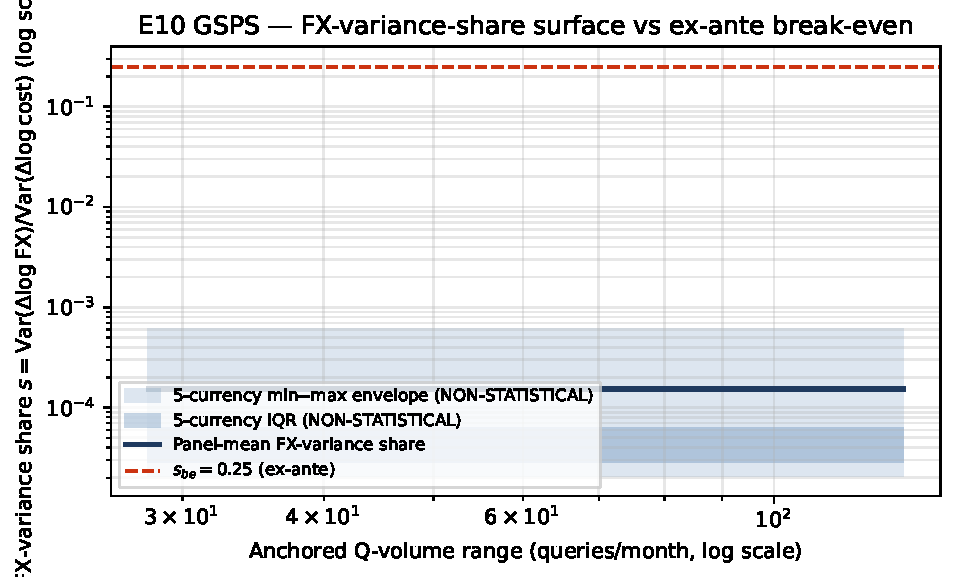
\includegraphics[width=0.92\linewidth]{figures/e10_figure1_surface_vs_break_even.pdf}
\caption{E10 GSPS FX-variance-share surface vs ex-ante-pinned break-even
  $\sbe = 0.25$, log-spaced 50-point grid across the anchored
  $[28, 130]$ queries/month range. The panel-mean surface
  ($\approx 1.535\times 10^{-4}$, navy line) is approximately
  $3.21$ decades below $\sbe$ (red dashed) at every grid point.
  The shaded bands are the 5-currency non-statistical envelope (min/max
  light; IQR darker). \textbf{DESCRIPTIVE / CALIBRATION-CONDITIONAL.}
  NOT a confidence interval. NOT an inferential band.}
\label{fig:e10-surface}
\end{figure}

\begin{figure}[h]
\centering
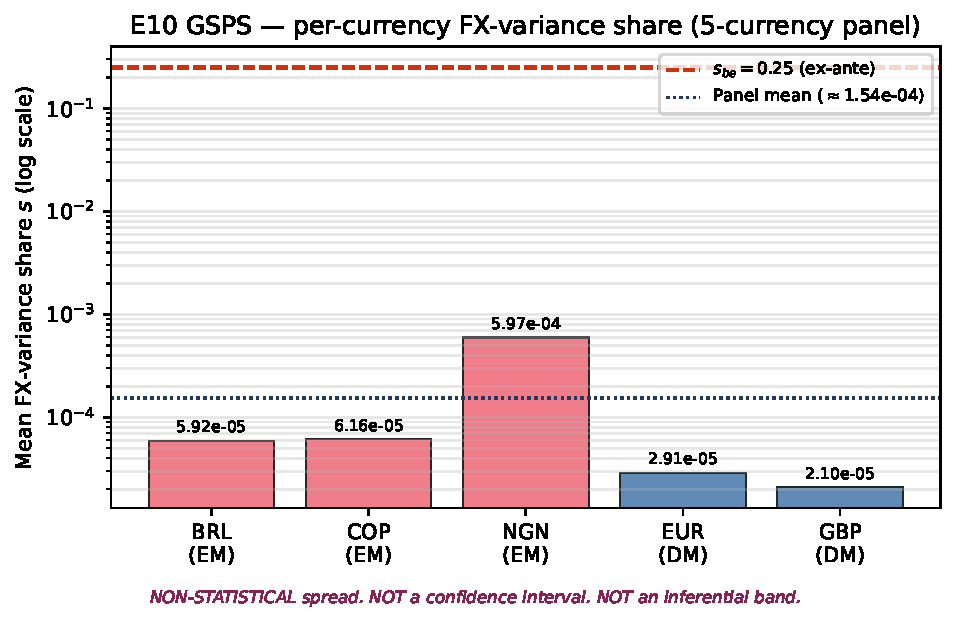
\includegraphics[width=0.92\linewidth]{figures/e10_figure2_currency_spread.pdf}
\caption{E10 GSPS per-currency mean FX-variance share over the 5-currency
  panel, EM (BRL/COP/NGN, salmon) vs DM (EUR/GBP, blue), against
  $\sbe = 0.25$ (red dashed) and the panel mean (navy dotted). All five
  currencies sit two to four decades below $\sbe$; NGN carries the largest
  share ($\approx 5.97\times 10^{-4}$, post-NFEM-float regime) and GBP the
  smallest ($\approx 2.10\times 10^{-5}$). \textbf{DESCRIPTIVE /
  NON-STATISTICAL spread.} NOT a confidence interval. NOT an inferential
  band.}
\label{fig:e10-currency-spread}
\end{figure}

\subsection{Sensitivity-arm concordance}
\label{sec:e10-arms-results}

Table~\ref{tab:e10-arms} summarizes the five pre-committed sensitivity
arms. Every arm preserves Q-variance dominance ($q\_dom$ flag = True) and
returns concordance verdict \texttt{concordant}; every concordance metric
sits well below the descriptive concordance threshold. The no-rescue
clause holds.

\begin{table}[h]
\centering
\caption{E10 GSPS --- sensitivity-arm concordance summary
  (descriptive only; per spec \S9 no-rescue clause, no arm can flip
  the primary verdict).}
\label{tab:e10-arms}
\small
\begin{tabular}{llcll}
\toprule
Arm & Concordance metric & $q\_dom$ flag & Verdict & Panel-mean share \\
\midrule
(b) Q--FX coupling             & $0.000$                       & True & concordant & $1.535\times 10^{-4}$ \\
(c) NGN break-window           & $4.04\times 10^{-5}$          & True & concordant & $1.131\times 10^{-4}$ \\
(d) GBM / JD comparator        & $3.41\times 10^{-5}$          & True & concordant & $1.876\times 10^{-4}$ \\
(e) Per-currency split         & $9.43\times 10^{-5}$          & True & concordant & $5.922\times 10^{-5}$ \\
(f) Q\_high extended           & $2.71\times 10^{-20}$         & True & concordant & $1.535\times 10^{-4}$ \\
\bottomrule
\end{tabular}
\end{table}

\subsection{Headline numerics}
\label{sec:e10-headline}

The vol-on-vol regression returns
$\hat\beta_{\mathrm{two\text{-}way}} = +68.151$ (currency FE $+$ month FE)
and $\hat\beta_{\mathrm{currency\text{-}only}} = +54.715$ (currency FE only,
co-primary). The descriptive gap is
$\hat\beta_{\mathrm{two\text{-}way}} - \hat\beta_{\mathrm{currency\text{-}only}}
= +13.436$, with sign concordance preserved across both co-primary FE
specifications; the magnitude differential is approximately 20\% of the
smaller coefficient. The descriptive sign gate of pre-pin field 1 holds.
The descriptive gap is interpretive content for the \S13 M-sketch
hedge-sizing step in the spec --- specifically the load on the
\emph{idiosyncratic} (within-month, cross-currency) component of FX-vol
exposure relative to the \emph{global} (month-shock-absorbed) component.

The panel-mean FX-variance share is $\bar s = 1.535\times 10^{-4}$ across the
150-cell panel, approximately $3.21$ decades below $\sbe = 0.25$ at
every grid point of the anchored $[28, 130]$ Q-range. Combined with the
unanimously concordant sensitivity arms, the verdict is
\textsc{Non-Retirement}, subtype \texttt{q\_dominance}.

% =====================================================================
\section{Interpretation (post-Keynesian theoretical frame)}
\label{sec:e10-interpretation}

The interpretive content of \S\ref{sec:e10-interpretation} is
\emph{interpretive prose only} and is explicitly labeled as such. It is not
a hypothesis test; it does not predict the \textsc{Non-Retirement} verdict
post-hoc; it explains the mechanistic verdict in post-Keynesian (PK) terms.

The Bhaduri--Laski--Riese (BLR) virtual-vs-real dichotomy
\citep{BhaduriLaskiRiese2006} frames financialization as a structural gap
between the virtual economy (asset valuation, financial-cycle volatility)
and the real economy (output, productive investment). The Minsky two-price
theory \citep{Tymoigne2010,Minsky1975} formalizes the gap between
$P_k$ (asset-side demand price) and $P_i$ (output-side supply price). The
Kaleckian investment-driven growth tradition
\citep{Kalecki1971,BhaduriMarglin1990} insists that investment, not asset
revaluation, is the prime mover of output.

The E10 representative Web3 data-analyst is a cohort whose cost-stream is
bound to its own activity intensity ($Q$, the own-output behavior --- the
$P_i$ side) rather than to virtual-economy price volatility ($\Cfx$ --- the
$P_k$ side). Under the calibration in Assumption~\ref{ass:A2}, on the
$[28, 130]$ anchored Q-range, the empirical FX-variance share sits
approximately three decades below the ex-ante break-even, indicating that
the convex FX hedge addresses the wrong variance vector for this cohort.
\emph{Calibration-conditional reading: all four PK bullets below are
interpretive prose for the configuration in pre-pin fields 1--7 of
Table~\ref{tab:e10-prepin}.}

\begin{itemize}
\item \textbf{BLR virtual-vs-real:} The convex FX hedge addresses the
  virtual-economy price-volatility vector ($P_k$ analog --- FX is the
  on-chain analog of virtual-economy price volatility); the cohort's
  cost-stream variance is structurally bound to the real-economy
  production decision (the analyst's $Q$ scheduling).
\item \textbf{Minsky two-price:} The instrument prices into the $P_k$ gap
  but the cohort's exposure lives on the $P_i$ side.
\item \textbf{Kaleckian:} The cohort's cost-stream variance reflects
  effective-demand-driven activity intensity, not asset-revaluation flow.
\item \textbf{Methods-paper hook:} The detection methodology survives the
  specific verdict --- it correctly routes this (cohort, instrument) pair
  to \textsc{Non-Retirement} subtype \texttt{q\_dominance} from
  public-source data alone, and the trail is auditable end-to-end.
\end{itemize}

The verdict is not a bug of the data and not a failure of the convex hedge
instrument family; it is a finding about the (cohort, instrument) pair.

% =====================================================================
\section{Methodology contribution survives the verdict}
\label{sec:e10-contribution}

The contribution of this section is the \emph{methodology}, not the
specific E10 verdict. The methodology successfully identifies:

\begin{enumerate}[label=(\alph*)]
\item a cohort whose cost-stream variance is Q-dominated under a
  NON-FANTASY simulator anchor and a frozen ex-ante break-even
  (Assumption~\ref{ass:A2}, Assumption~\ref{ass:A5});
\item an instrument (the convex FX hedge) that addresses the wrong
  variance vector for that cohort, with the dominance gap quantified at
  more than three decades below the ex-ante threshold;
\item the verdict ladder (Algorithm~\ref{alg:ladder}) routing this
  (cohort, instrument) pair to \textsc{Non-Retirement} subtype
  \texttt{q\_dominance};
\item an auditable trail --- Tier-2-frozen central-bank data with
  payload-SHA-256 provenance sidecars; NON-FANTASY simulator anchor
  against 214 genuine observed tool calls; the exact \S\ref{sec:e10-decomposition}
  identity at machine precision; an ex-ante-pinned break-even derived
  before any decomposition runs.
\end{enumerate}

The methodology is venue-publishable as a stand-alone Section~5 of a
methods paper at \emph{Cambridge Journal of Economics}, \emph{Review of
Political Economy}, or \emph{Metroeconomica} independent of the specific
E10 verdict. The companion sections of the methods paper apply analogous
detection methodologies to alternative (cohort, instrument) pairs (E8
dTAO/Maymin; E9 LATAM RWA) and are reported separately.

% =====================================================================
\section{Limitations and future iterations}
\label{sec:e10-limitations}

The methodology, as deployed in E10, carries the following honest
limitations:

\begin{itemize}
\item \textbf{Q-FX coupling is an algebraic-identity assertion under the
  user-pinned operationalization, not a coupled-daily re-simulation.}
  The arm (b) operationalization rescales monthly Q magnitudes by a single
  per-month scalar; a constant scalar drops out of daily $\dln Q$ within
  the month, so the within-month log-variance decomposition is unchanged
  at the cell level. The arm reports this transparently. A coupled-daily
  re-simulation would be a natural extension.

\item \textbf{The FX-variance-share surface is panel-mean-invariant in Q
  for the E10 calibrated simulator.} The implementation broadcasts the
  panel-mean share to every grid point and emits an
  \texttt{is\_panel\_mean\_broadcast} flag so consumers cannot read the
  surface as an estimated Q$\to s$ mapping. A kernel-smoothed
  Q-volume-dependent surface (a non-parametric regression of $s$ on $Q$
  across cells) would be a natural follow-up.

\item \textbf{$G = 5$ currency clusters is structurally thin.}
  Cluster-robust inference at $G = 5$ is size-distorted; we report
  descriptive sign and non-statistical min--max / IQR spreads only.
  Bootstrap-based bands were considered and dropped at this $G$ in spec
  v0.6 (CORRECTIONS-E10-6).

\item \textbf{The arm (d) GBM/JD comparator's calibration is per-step
  rather than monthly-aggregate.} The Geometric-Brownian-Motion and
  Merton-Jump-Diffusion generators interpret \texttt{sigma\_per\_month} as
  a per-step variance target; the simulated per-step
  $\Var(\dln \Cfx_{\mathrm{sub}})$ differs from the target
  monthly-aggregate $\Var(\Sigma\,\dln \Cfx)$ by a factor proportional to
  $1 / n_{\mathrm{steps}}$. The deflation does not flip the verdict ---
  arm (d) remains concordant --- but the comparator-moment description is
  not naively the panel-mean FX variance and is reported here for
  transparency.

\item \textbf{The \texttt{\_MIN\_SURVIVING\_DAYS} threshold of 2 in the
  cell-decomposition function is methodologically degenerate.} At $n = 2$
  surviving days only one daily log-return exists; the population variance
  of a one-element series is zero. All 150 production cells have
  $\gg 3$ surviving days, so this is benign in E10; a future amendment
  would raise the threshold to 3 (one degree of freedom for variance).

\item \textbf{The break-even threshold uses an ideal-scenario premium
  ($c_{\mathrm{payoff}} = 1$, $\varphi = 0.25$).} No FX-stablecoin
  options venue with real depth exists in 2026; a real venue would impose
  $c_{\mathrm{payoff}} < 1$ and lift $\sbe$ above $0.25$. The frozen
  $\sbe = 0.25$ is the ideal-scenario lower bound on the break-even share.

\item \textbf{The methods-paper §5 hook is robust across alternative
  cohort / instrument pairings.} E8 dTAO/Maymin and E9 LATAM RWA are
  companion sections of the joint outline; the detection methodology
  applies analogously.
\end{itemize}

% =====================================================================
\section*{References}
\begin{thebibliography}{99}

\bibitem[Abrigo (2026)]{AbrigoSpecE10v07}
Abrigo Analytics (2026).
\newblock E10 GSPS v0.7: Convex Multi-Currency Data-Consumption FX-Volatility Hedge --- Design Specification.
\newblock \texttt{docs/specs/2026-05-20-e10-gsps-v0.7-convex-multicurrency-design.md}.

\bibitem[Bhaduri \& Marglin(1990)]{BhaduriMarglin1990}
Bhaduri, A. and Marglin, S. (1990).
\newblock Unemployment and the Real Wage: The Economic Basis for Contesting Political Ideologies.
\newblock \emph{Cambridge Journal of Economics}, 14(4), 375--393.

\bibitem[Bhaduri, Laski \& Riese(2006)]{BhaduriLaskiRiese2006}
Bhaduri, A., Laski, K. and Riese, M. (2006).
\newblock A Model of Interaction between the Virtual and the Real Economy.
\newblock \emph{Metroeconomica}, 57(3), 412--427.

\bibitem[Cox(1955)]{Cox1955}
Cox, D.~R. (1955).
\newblock Some Statistical Methods Connected with Series of Events.
\newblock \emph{Journal of the Royal Statistical Society, Series B}, 17(2), 129--164.

\bibitem[Kalecki(1971)]{Kalecki1971}
Kalecki, M. (1971).
\newblock \emph{Selected Essays on the Dynamics of the Capitalist Economy 1933--1970}.
\newblock Cambridge University Press.

\bibitem[Lambert, Lyons \& Jiao(2022)]{LambertLyonsJiao2022}
Lambert, G., Lyons, J. and Jiao, J. (2022).
\newblock Panoptic: A Perpetual, Oracle-free Options Protocol.
\newblock arXiv:2204.14232.

\bibitem[Lambert(2022)]{Lambert2022Panoptic}
Lambert, G. (2022).
\newblock Static replication of arbitrary payoffs by portfolios of perpetual options.
\newblock Panoptic Working Paper.

\bibitem[Maymin(2026)]{Maymin2026}
Maymin, P. (2026).
\newblock A CEV-based Process for AMM Tokens with Closed-form Option Pricing.
\newblock arXiv:2603.29763.

\bibitem[Merton(1976)]{Merton1976}
Merton, R.~C. (1976).
\newblock Option Pricing when Underlying Stock Returns are Discontinuous.
\newblock \emph{Journal of Financial Economics}, 3(1--2), 125--144.

\bibitem[Mento Labs(2024)]{Mento2024}
Mento Labs (2024).
\newblock Mento Protocol --- Reserve, Stability Mechanism, and FX-Stablecoin Catalog.
\newblock \texttt{https://www.mento.org/}.

\bibitem[Minsky(1975)]{Minsky1975}
Minsky, H.~P. (1975).
\newblock \emph{John Maynard Keynes}.
\newblock Columbia University Press.

\bibitem[Tymoigne(2010)]{Tymoigne2010}
Tymoigne, E. (2010).
\newblock Minsky's Two-Price Theory of Investment.
\newblock Levy Economics Institute Working Paper.

\bibitem[x402 Working Group(2025)]{x402Spec}
x402 Working Group (2025).
\newblock x402: HTTP 402 Revival --- Per-request Payment Protocol Specification.
\newblock Linux Foundation Governance.

\end{thebibliography}

\end{document}
